\documentclass[11pt]{article}

%imports
\usepackage[utf8]{inputenc}
\usepackage[T1]{fontenc}
\usepackage{amsmath}
\usepackage{amsfonts}
\usepackage{amssymb}
\usepackage{footnote}
\usepackage{url}
\usepackage{hyperref}
\usepackage{subcaption}
\usepackage{tikz}
\usepackage{amsthm}
\usepackage{longtable}

\usetikzlibrary{fit,shapes.geometric}


%images and image path
\usepackage{graphicx}
%\usepackage{subfig}
\graphicspath{ {./images/} }

%custom commands
\newcommand{\R}{\mathbf{R}}
\newcommand{\C}{\mathbf{C}}
\newcommand{\N}{\mathcal{N}}
\newcommand{\num}{\text{num}}
\newcommand{\obs}{\text{obs}}
\newcommand{\D}{\mathfrak{D}}
\newcommand{\Ro}{\mathcal{R}_0}
\newcommand{\lap}{{\mathcal{L}}}
\renewcommand\vec{\mathbf}
\newcommand{\mat}[1]{\mathsf{#1}}
\newcommand{\U}{\mathcal{U}}

\newtheorem{theorem}{Theorem}
\newtheorem{conjecture}{Conjecture}
\newtheorem{definition}{Definition}

%intsitute command
\usepackage{etoolbox}
\makeatletter
\providecommand{\institute}[1]{% add institute to \maketitle
	\apptocmd{\@author}{\end{tabular}
	\par
	\begin{tabular}[t]{c}
		\small \textit{#1}}{}{}
}
\makeatother

%margins
\usepackage[letterpaper, total={6.5in, 9.5in}]{geometry}

%opening
\title{Reaction-diffusion spatial modeling of COVID-19 in Chicago}
\author{Trent Gerew\thanks{\texttt{tgerew@hawk.iit.edu}}}
\institute{Department of Applied Mathematics, Illinois Institute of Technology, Chicago, Illinois}

\begin{document}

\maketitle

\begin{abstract}
	content...
\end{abstract}

\section{Introduction}

\section{Materials and methods}
	\subsection{Confirmed and death data}
		In this study, we used the publicly available data set of COVID-19 provided by the City of Chicago Data Portal \cite{Chicago-cases}.
		This data set includes daily counts of confirmed infected cases, hospitalizations, and deaths.
	
	\subsection{Mathematical model}
		We focus our study on four components of the epidemic flow (Figure \ref{fig:model}).
		That is, the populations of Susceptible individuals ($S$), Asymptomatic infected individuals ($A$), symptomatic Infected individuals ($I$), and Removed individuals ($R$).
		\begin{figure}[h]
			\centering
			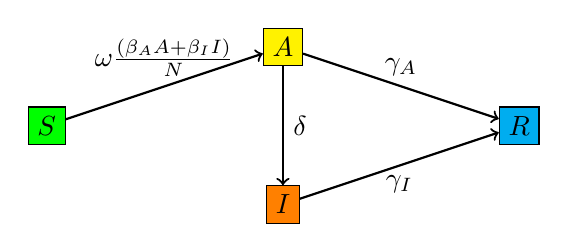
\begin{tikzpicture}
				\node[shape=rectangle, draw=black, fill=green] (s) at (-3,0) {$S$};
				\node[shape=rectangle, draw=black, fill=yellow] (a) at (0,1) {$A$};
				\node[shape=rectangle, draw=black, fill=orange] (i) at (0,-1) {$I$};
				\node[shape=rectangle, draw=black, fill=cyan] (r) at (3,0) {$R$};
				\path[thick,->] (s) edge node[above,swap] {$\omega \frac{(\beta_A A + \beta_I I)}{N}$} (a);
				\path[thick,->] (a) edge node[right,swap] {$\delta$} (i);
				\path[thick,->] (a) edge node[above,swap] {$\gamma_A$}	(r);
				\path[thick,->] (i) edge node[below,swap] {$\gamma_I$}	(r);
			\end{tikzpicture}
			\caption{Compartmental representation of the SAIR model.}
			\label{fig:model}
		\end{figure}
		Our model is known as the SAIR model \cite{s+t+spain}, which substitutes the $E$ compartment of the SEIR model by the $A$ compartment.
		This model is relevant when there are many undetected asymptomatic infectious individuals, which is known to be the case for COVID-19.
		
		We motivate the use of this simple model for the following reasons:
		\begin{itemize}
			\item
				We do not consider the $E$ group in this work because we feel this population can be merged with the $A$ group.
			\item
				We do not distinguish between quarantined, hospitalized, or nursing-home populations.
				Including these additional compartments would over parameterize the model.
				Additionally, the way in which data has been collected and is provided by authorities has varied over time, making its usage rather difficult \cite{sara-data}.
				For the same reasons, we do not distinguish between deceased and recovered.
		\end{itemize}
	
		To build the mathematical model, we followed the standard strategy developed in the literature concerning SIR models \cite{bio-models}.
		We assume that individuals in $S$ can be infected by both members of $A$ and $I$.
		We suppose that the individuals in the $A$ and $I$ compartments may have different contact rates $\beta_A$ and $\beta_I$, and different recovery rates $\gamma_A$ and $\gamma_I$.
		Furthermore, we consider a rate $\delta$ at which individuals in $A$ may develop symptoms or are otherwise detected and so will move to the $I$ compartment.
		Lastly, we assume that only members of $S$ and $A$ are mobile.
		
		The dynamics is governed by a system of two partial differential equations (PDE) and two ordinary differential equations (ODE) as follows, for $\vec{x} = (x,y) \in \Omega \subset \R^2, t > 0$,
		\begin{equation} \label{eq:model}
			\begin{aligned}
				\partial_t S - D(t) \Delta S &= - \omega(t) \frac{\beta_A A + \beta_I I}{N} S, \\
				\partial_t A - D(t) \Delta A &= \omega(t) \frac{\beta_A A + \beta_I I}{N} S - (\gamma_A - \delta) A, \\
				I' &= - \gamma_I I + \delta A, \\
				R' &= \gamma_A A + \gamma_I.
			\end{aligned}
		\end{equation}
		Since travel into the city of Chicago was heavily restricted for the early stages of the pandemic, the homogeneous Neumann boundary condition is imposed \cite{Mammeri+2020+102+113}.
		The total population is $N = S + A + I + R$, and is considered a constant.
	
	\subsection{Parameter estimation}
		To account for the lockdown, the average number of of contacts is updated as follows \cite{Kevrekidis-2021}
		\begin{equation} \label{eq:contacts}
			\omega (t) = \omega_0 \left[ \eta + (1 - \eta) \frac{1 - \tanh \left[2 (t - t_q) \right]}{2} \right],
		\end{equation}
		while the diffusion coefficient is similarly
		\begin{equation} \label{eq:diffusion}
			D (t) = D_0 \left[ \eta + (1 - \eta) \frac{1 - \tanh \left[2 (t - t_q) \right]}{2} \right].
		\end{equation}
		Here, $t_q = (t_{\mathrm{eol}} + t_{\mathrm{bol}}) / 2$, where $\mathrm{bol}$ denotes the beginning of the lockdown and $\mathrm{eol}$ denotes the end of the lockdown.
		The parameter $0 \leq \eta \leq 1$ is a varying coefficient translating respect for social distancing and other preventative measures.
		Note that $\omega_0$ is the average number of contacts before any intervention, and is a constant.
	
	\subsection{Numerical discretization}
	
\section{Results}
	\subsection{Existence of solutions and basic reproduction numbers}
		We show that we are justified in searching for suitable parameters to solve the model.
		Let $\vec{x} = (S,  A, I, R)$ and $\vec{x}_0 = (S_0, A_0, I_0, R_0)$.
		First we show that the solution of the initial value problem (\ref{eq:model}) exists for the case with no diffusion.
		\begin{theorem}
			Let $0 \leq \vec{x}_0 \leq N$ be the initial datum.
			Then there exists a unique in time solution $\vec{x}$ of the initial value problem (\ref{eq:model}) without diffusion over $C \subset U \subset \R^4 \times \R^1$ where $C$ is a compact set that contains $(\vec{x}_0, t_0)$.
			Moreover, the solution is $\C^1$.
		\end{theorem}
		\begin{proof}
			Since $\vec{x}_t = f(\vec{x},t)$ is $\C^1$ on the open set $U \subset \R^4 \times \R^1$, it follows that there exists a solution of (\ref{eq:model}) without diffusion through the point $\vec{x}_0$ at $t = t_0$ for $|t - t_0|$ sufficiently small.
			Moreover, $\vec{x} (t, t_0,\vec{x_0})$ is a $\C^1$ function \cite{dynamics}.
			Since $C$ is a compact set containing $(\vec{x}_0, t_0)$, then the solution $\vec{x} (t, t_0, \vec{x}_0)$ can be uniquely extended backward and forward in $t$ up to the boundary of $C$ \cite{dynamics}.
		\end{proof}
		\noindent We do provide a proof for the existence of solutions to the initial boundary value problem (\ref{eq:model}) with diffusion terms, but we assume it exists.
		\begin{conjecture}
			Let $0 \leq \vec{x}_0 \leq N$ the initial datum.
			Then there exists a unique global in time solution $\vec{x}$ of the initial boundary value problem (\ref{eq:model}).
		\end{conjecture}
		\noindent A proof for this conjecture will be similar to the one given in \cite{Mammeri+2020+102+113}.
		
		An important parameter in understanding the initial growth of the virus is the basic reproduction number.
		\begin{definition}[Basic Reproduction Number]
			The basic reproduction number $\Ro$ can be computed using the next generation of the model without diffusion.
			Since the infected individuals are in $A$ and $I$, new infections ($\mathcal{F}$) and transitions between compartments ($\mathcal{V}$) can be rewritten as
			\begin{align*}
				\mathcal{F} &= \begin{pmatrix} \omega (\beta_A A + \beta_I I) \frac{S}{N} \\ 0 \end{pmatrix}, &
				\mathcal{V} &= \begin{pmatrix} (\gamma_A + \delta) A \\ \gamma_I - \delta A \end{pmatrix}.
			\end{align*}
			Thus, $\Ro = \rho (\mat{F} \mat{V}^{-1})$ of the next generation matrix
			\begin{equation*}
				\mat{F} \mat{V}^{-1} = \begin{pmatrix} 
				\frac{S_0 \omega_0 \beta_A}{N (\gamma_A + \delta)} + \frac{S_0 \omega_0 \beta_I \delta}{N \gamma_I (\gamma_A + \delta)} & 
				\frac{S_0 \omega_0 \beta_I}{N \gamma_I} \\ 
				0 & 0 \end{pmatrix}.
			\end{equation*}
			So,
			\begin{equation} \label{eq:ro}
				\Ro =  \frac{\omega_0}{\gamma_A + \delta}  \left( \beta_A + \beta_I \frac{\delta}{\gamma_I} \right) \frac{S_0}{N}.
			\end{equation}
		\end{definition}
		\noindent This number is dimensionless and has an epidemiological meaning.
		The first term represents the transmission rate by asymptomatic individuals, and the second term represents the transmission rate by symptomatic individuals.
			
	\subsection{Model resolution}
	
	\subsection{Spatial spread of COVID-19}

\section{Discussion}
	
	\textbf{Acknowledgments:} \\
	\textbf{Funding:}
	This research was funded by the Socially Responsible Modeling, Computation, and Design (SoReMo) Initiative, at the Illinois Institute of Technology. \\
	\textbf{Conflicts of Interest:}
	
\section*{Appendix}
	\subsection*{Nomenclature (Units are indicated in brackets.)}
		\begin{longtable}{c l l}
			\textbf{Latin symbols} & & \\
			$A$ & Asymptomatic infected individuals & [individuals] \\
			$D$ & Diffusivity & \\
			$I$ & Symptomatic infected individuals & [individuals] \\
			$N$ & Total population of individuals & [individuals] \\
			$R$ & Removed individuals & [individuals] \\
			$S$ & Susceptible individuals & [individuals] \\
			\textbf{Greek symbols} & & \\
			$\beta_j$ & Contact rate of compartment $j$ & [days\textsuperscript{-1}] \\
			$\gamma_j$ & Recovery rate of compartment $j$ & [days\textsuperscript{-1}] \\
			$\delta$ & Rate of asymptomatic individuals that may develop symptoms & [days\textsuperscript{-1}] \\
			$\omega$ & Contacts & 
		\end{longtable}
\bibliographystyle{abbrv}
\bibliography{version3}

\end{document}
